\section{\lr{fine tuning}}

\subsection{مدل زبانی}
از بین 12 ژانر موجود؛ 6 ژانر اول با بیشترین تعداد جمله برای تسک 
\lr{fine-tune}
انتخاب شدند. در این قسمت از کد
\lr{huggingface}
\cite{Ref1}
و مدل 
\lr{Distil GPT2}
برای 
\lr{fine-tune}
روی داده هر کلاس  استفاده شده است. مدل زبانی هر ژانر از نوع
\lr{causal}
است و برای 6 دور با
\lr{batch size}
1000
\lr{fine-tune}
می شود. همچنین داده هر ژانر به نسبت 80 به 20 به دو قسمت آموزش و ارزیابی تقسیم می شود. از داده ارزیابی در زمان 
\lr{fine-tune}
و در پایان برای اندازه گیری
\lr{perplexity}
استفاده می شود. از دیگر تنظیمات مدل می توان به اعمال
\lr{weight decay}
و توقف زودهنگام (\lr{early stopping}) اشاره کرد. مقایسه perplexity مدل ها در جدول
\ref{tab51}
آورده شده است. از آنجایی که زمان 
\lr{fine-tune}
کوتاه بوده و تعداد جملات برای هر ژانر زیاد نیست، perplexity ها مقادیر خوبی ندارند.


\begin{center}
	\begin{table}
		\begin{center}
		\begin{tabular}{ |c|c| }
		\hline
		\textbf{Genre} & \textbf{Perpelexity} \\ 
		\hline
		Action  & $\input{../report/fine_tuning/Action_bert_lm/perplexity.txt} $ \\
		\hline
		Adventure  & $\input{../report/fine_tuning/Adventure_bert_lm/perplexity.txt} $ \\
		\hline
		Fantasy  & $\input{../report/fine_tuning/Fantasy_bert_lm/perplexity.txt} $ \\
		\hline
		Drama & $\input{../report/fine_tuning/Drama_bert_lm/perplexity.txt} $ \\
		\hline
		Comedy  & $\input{../report/fine_tuning/Comedy_bert_lm/perplexity.txt} $ \\
		\hline
		Romance  & $\input{../report/fine_tuning/Romance_bert_lm/perplexity.txt} $ \\
		\hline
	\end{tabular}
\caption{\label{tab51}مقایسه perplexity مدل زبانی ژانرها \lr{fine-tune}}
\end{center}
\end{table}
\end{center}

تعدادی از جملات تولید شده توسط مدل ها در جدول \ref{tab52} بررسی شده اند. کلمات آبی شده توسط مدل تولید شده اند. کلمات ناقص به دلیل حذف کردن stopwords از داده اصلی به وجود آمده اند. در این مثال ژانرهای 
\lr{Action}،
\lr{Adventure}
و
\lr{Drama}
جملات مناسب و مرتبطی تولید کرده اند.



\begin{center}
	\begin{table}
		\begin{center}
			\begin{tabular}{ |c|c| }
				\hline
				\textbf{Genre} & \textbf{Sentence} \\ 
				\hline
				Action  & \lr{ an accident \textcolor{blue}{ NUM year ago left mrunas} }\\
				\hline
				Adventure  & \lr{ an accident \textcolor{blue}{dimension finally meet fate new member group come}} \\
				\hline
				Fantasy  & \lr{ an accident \textcolor{blue}{happens people think wrongperson named ik}} \\
				\hline
				Drama & \lr{  an accident \textcolor{blue}{set fire inside roomtakanagi}} \\
				\hline
				Comedy  & \lr{  an accident \textcolor{blue}{also happens accidentally end yukichi girl}} \\
				\hline
				Romance  & \lr{ an accident \textcolor{blue}{dimension world called nanamiunusual day}} \\
				\hline
			\end{tabular}
			\caption{\label{tab52}مقایسه جملات تولید شده \lr{fine-tune}}
		\end{center}
	\end{table}
\end{center}


در مثال دوم در جدول
\ref{tab53}
جمله تولید شده توسط ژانرهای 
\lr{Action}،
\lr{Adventure}
و
\lr{Fantasy}
کاملا حال و فضای ژانر را دارد و بقیه ژانرها نیز به نسبت کلمات مناسبی تولید کرده اند.

	\begin{table}
		\begin{center}
			\begin{tabular}{ |c|c| }
				\hline
				\textbf{Genre} & \textbf{Sentence} \\ 
				\hline
				Action  & \lr{ he was from \textcolor{blue}{far away girl come new world} }\\
				\hline
				Adventure  & \lr{ he was from \textcolor{blue}{the previous generation ai japan}} \\
				\hline
				Fantasy  & \lr{ he was from \textcolor{blue}{another dimension time travel another dimension new}} \\
				\hline
				Drama & \lr{ he was from \textcolor{blue}{hino one day find dead another}} \\
				\hline
				Comedy  & \lr{he was from \textcolor{blue}{ home village made thing even worsehow}} \\
				\hline
				Romance  & \lr{he was from \textcolor{blue}{heaven told never say anything one day}} \\
				\hline
			\end{tabular}
			\caption{\label{tab53}مقایسه جملات تولید شده \lr{fine-tune}}
		\end{center}
	\end{table}

در مجموع جملات تولید شده توسط مدل های 
\lr{fine-tune}
شده، کیفیت و خوانایی بهتری نسبت به مدل های قسمت قبل دارد که این نشان دهنده مزایای استفاده از مدل های از پیش آموزش دیده است. مثال های آورده شده از مجموعه پیش بینی های مدل ها دستچین شده اند. فایل کامل کلمات تولید شده توسط هر مدل با اسم 
\textit{predictions.txt}
در پوشه 
\textit{reports}
قرار دارد.


\subsection{رده بندی}

چالش رده بندی ژانر بر اساس خلاصه انیمه 
\lr{multilabel classification}
نام دارد. در این قسمت هر خلاصه 12 برچسب دارد و بر پایه اینکه یک ژانر به این خلاصه تعلق داشته باشد مقدار صفر یا یک می گیرد \cite{Ref2}. مدل 
\lr{bert-base-uncased}
 برای 4 دور با تکنیک 
 \lr{cross validation}
 و تابع خطا 
 \lr{binary cross entropy}
 آموزش می بیند. در پایان آموزش دقت مدل روی داده 
 \lr{validation}
 $18.52$
 و
 \lr{F1 score}
 آن 
 $58.67$
 است.
 
 شکل \ref{fig51} عملکرد مدل را روی داده تست نشان می دهد. پارامتر
 support
 نشان دهنده تعداد خلاصه ها با یک ژانر مشخص هستند. بیشترین دقت متعلق به ژانر
 Romance
 است چون این ژانر بیشترین تعداد خلاصه را دارد. ژانر های 
 \lr{School life}
 و
 \lr{Fantasy}
 نیز دقت بالایی دارند که می تواند به دلیل شباهت یا همراه بودن با ژانر 
 Romance
 باشد (انیمه هایی که ژانر Romance دارند اکثر ژانرهای
 \lr{School life}
 و
 \lr{Fantasy}
 نیز دارند). ژانر 
 Drama
 دقت و recall
 پایینی دارد. دلیل آن می تواند برجسته نبودن ژانر
 Drama
 باشد، به عبارت دیگر در مقایسه با ژانر 
 \lr{Action}
 یا
 Romance
 که کلمات مشخصی از قبیل 
 fight 
 یا
 love
 دارند، این ژانر کلمات مشخصی ندارد به همین دلیل تشخیص آن سخت تر است. ژانر
 \lr{Sci Fi}
 نیز به دلیل کم بودن تعداد داکیومنت ها 
recall
پایینی دارد که با افزایش داده می توان این مشکل را حل کرد. فایل 
\textit{comparisons.csv}
تمام پیش بینی ها و برچسب های درست برای داده تست نشان می دهد.
 
 
 \begin{figure}[H]
 	\centering
 	
 	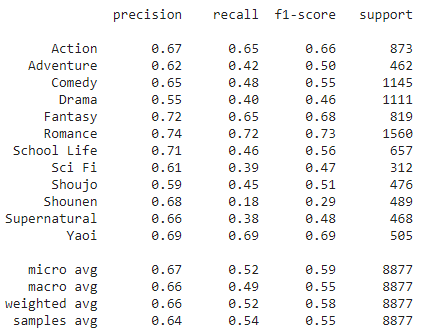
\includegraphics[width=0.8\textwidth,height=0.8\textheight,keepaspectratio]{images/5-1}
 	\caption{عملکرد مدل رده بند روی داده تست}
 	\label{fig51}
 	
 \end{figure} 
 

